\documentclass[red]{beamer}

\mode<presentation>
{
  \usetheme{Antibes}
  \usecolortheme{dolphin}
  \setbeamertemplate{footline}[frame number]
}

\usepackage[english]{babel}
\usepackage{subfigure}
\usepackage{xunicode}
\usepackage{xltxtra}
\usepackage{fontspec}
\usepackage{wrapfig}
\usepackage{subfigure}
\setmainfont{Ubuntu}

\title
{Image Based Flow Visualization \\
}

\author
{Jeroen Hofman}

\institute
{
 Department of Computational Science\\
 University of Amsterdam}

\pgfdeclareimage[height=0.8cm]{university-logo}{logo.png}
\logo{\pgfuseimage{university-logo}}

\begin{document}
\graphicspath{{/home/jhofman/Desktop/CSS/Figures/}}
\setbeamertemplate{navigation symbols}{}


\begin{frame}
  \titlepage
\end{frame}

\begin{frame}
  \begin{center}
    Based on \\
    \emph{Image Based Flow Visualization} \\
    by J. van Wijk \\
    \vspace{10pt}
    \small{ACM Transaction on Graphics (TOG) -\\ Proceedings of ACM SIGGRAPH 2002,\\ July 2002, Vol. 21, No. 3, 745-754}
  \end{center}
\end{frame}

\begin{frame}{Introduction}
  \begin{itemize}
  \item 
    Fluid flow is dominant in many fields, for instance climate prediction, industrial processes, thermodynamic flows etc. Animation is crucial for physical insight.
  \item
    Computations are usually done on large data-sets and high resolutions.
  \item
    The method proposed by the author produces efficient visualizations of \emph{unsteady flows}.
  \end{itemize}
\end{frame}


\begin{frame}{Basic Idea}
  Basic idea for \emph{Image Based Flow Visualization} (IBVF):
  \begin{figure}[H]
    \centering
    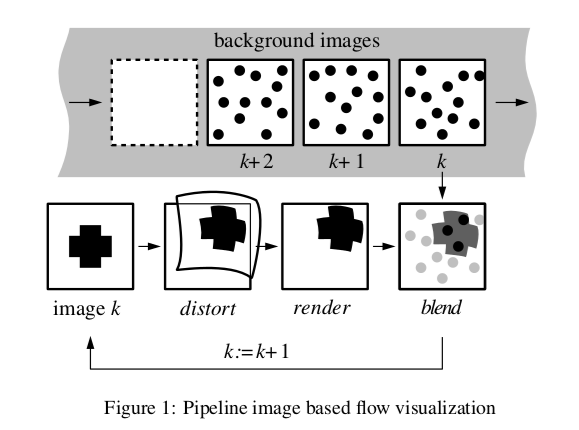
\includegraphics[width=0.6\textwidth]{pipeline.png}
  \end{figure}
\end{frame}

\begin{frame}{Formal Setup}
  $\boldsymbol{v}(\boldsymbol{x},t) \in S \subset \mathbb{R}^2$\\
  \vspace{10pt}
  Path lines $\boldsymbol{p}(t)$, following $d\boldsymbol{p}(t)/dt = \boldsymbol{v}(\boldsymbol{p}(t),t)$.\\
  \vspace{10pt}
  For a field (image) $F(\boldsymbol{x},k)$ representing some property of the flow we have:
  \begin{equation*}
    F(\boldsymbol{p}_{k+1},k+1) = \begin{cases} F(\boldsymbol{p}_{k},k) \; \text{if} \; \boldsymbol{p}_k \in S \\
      0 \; \text{otherwise}
      \end{cases}
  \end{equation*}
  \textbf{Problem}: this leads to an empty (black) space.
\end{frame}

\begin{frame}{Formal Setup}
  \textbf{Solution}: blend with background.
  \begin{equation*}
    F(\boldsymbol{p}_{k},k) = (1 - \alpha) F(\boldsymbol{p}_{k-1},k-1) + \alpha G(\boldsymbol{p}_k,k)
  \end{equation*}
  where $\alpha$ is called the \emph{blending mask}.\\
  \vspace{5pt}
  If we write out the recurrence:
  \begin{equation*}
    F(\boldsymbol{p}_{k},k) = \alpha \sum^{k-1}_{i=0} (1 - \alpha)^i G(\boldsymbol{p}_{k-i},k-i)    
  \end{equation*}
\end{frame}

\begin{frame}{Background Image Generation}
  What type of background images should be used?\\
  \vspace{10pt}
  Completely random: variation too strong and no streaming.\\
  \vspace{10pt}
  Make $G$ periodic:\\
  \begin{equation*}
    G_{i,k} = w((k/M + \phi_i) \mod 1)
  \end{equation*}
\end{frame}

\begin{frame}{Phase Profiles}
  Different phase profiles lead to different textures:
  \begin{figure}[H]
    \centering
    \subfigure{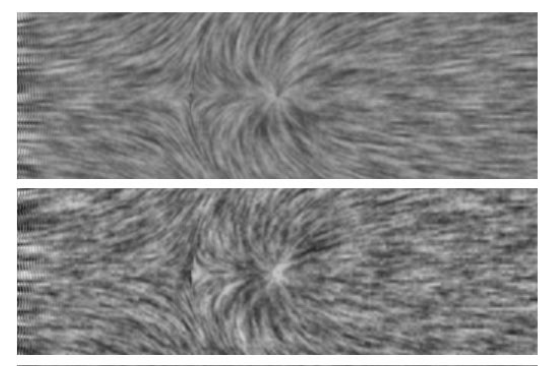
\includegraphics[width=0.45\textwidth]{profile1.png}}
    \subfigure{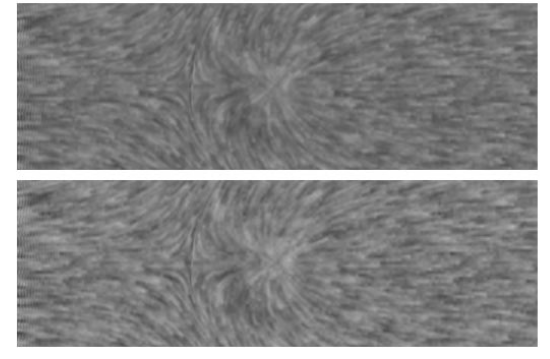
\includegraphics[width=0.45\textwidth]{profile2.png}}
    \caption{Results for different profiles: cosine (upper left), square (lower left), exponential decay (upper right), saw tooth (lower right).}
  \end{figure}
\end{frame}

\begin{frame}{Algorithm}
  \begin{itemize}
  \item 
    Calculate a distorted mesh $R$ according to flow lines (in case of unsteady flow).
  \item
    Render $R$, texture mapped with the previous image.
  \item
    Overlay a random noise pattern in the rectangle and blend with a factor $\alpha$, whereas the texture mapping of $R$ is blended with a factor $1 - \alpha$.
  \item
    Draw injected dye (if present).
  \item
    Render combined image on screen, together with overlay.
  \end{itemize}
\end{frame}


\begin{frame}{Results}
  See demo:
  \begin{itemize}
  \item 
    Meshes.
  \item
    Grid generation functions.
  \item
    Layouts (arrows, particles, topology, smeared, warped).
  \item
    Values for $\alpha$.
  \end{itemize}
\end{frame}


\begin{frame}{Efficiency}
  High degree of efficiency because of:
  \begin{itemize}
  \item 
    Highly optimized for use on graphics cards.
  \item
    Only 2 operations over the screen used per frame.
  \item
    Exploiting frame to frame coherence.
  \item
    Velocity field resolution is smaller than image resolution.
  \end{itemize}
\end{frame}

\begin{frame}{Developments}
  \begin{itemize}
  \item 
    IBFV model has been implemented in 3D.
  \item
    There are many methods using similar techniques like LEA, UFAC, UFLIC and many others. \\
    See website by Dr. Zhanping Liu.
  \end{itemize}

  \let\thefootnote\relax\footnotetext{\tiny{A. Telaru, J. van Wijk \emph{3D IBFV: Hardware-accelerated 3D Flow Visualization.}, 2003, Proceedings of the 14th IEEE Visualization Conference, 233-240}}
  \let\thefootnote\relax\footnotetext{\tiny{http://www.zhanpingliu.org/research/flowvis/auflic/comparison.html}}
\end{frame}

\begin{frame}{The End}
  \huge{Questions?}
\end{frame}

\end{document}